% @Author: AnthonyKenny98
% @Date:   2020-04-04 10:01:40
% @Last Modified by:   AnthonyKenny98
% @Last Modified time: 2020-04-04 11:17:14

A funny paradox in computer science is the fact that it is relatively easy to teach a computer to perform tasks that humans find very complicated, but extremely difficult to program one to execute functions that humans master during infancy. Consider, it was as early as 1949 that Claude Shannon presented his paper \textit{Programming a Computer for Playing Chess}\cite{Shannon1950}, and by 1997 the \textit{Deep Blue} computer defeated Garry Kasparov, reigning world champion, in a six game chess match.\cite{Campbell2002} Compare that with some of the most advanced autonomous humanoid robots to date displaying dexterity comparable with a toddler. The task of finding a collision free path, performed constantly without thought by a human, is an example of this paradigm. For a robot to compute a collision free path, it relies on a set of Motion Planning Algorithms.

Motion Planning Algorithms refer to the set of algorithms that find possible sequences of valid \gls{configuration}s for a robot in a space. In plain English, they are algorithms that determine the movements a robot can make in a map, with the intent of eventually finding a path from one point to another. 

\subsection{Key Concepts}

    \subsubsection{Configuration}

    % @Author: AnthonyKenny98
% @Date:   2020-04-04 11:13:58
% @Last Modified by:   AnthonyKenny98
% @Last Modified time: 2020-04-04 12:09:59
% @Author: AnthonyKenny98
% @Date:   2020-02-29 17:30:44
% @Last Modified by:   AnthonyKenny98
% @Last Modified time: 2020-04-03 14:28:30
\begin{figure}[H]
\begin{center}
\begin{tabular}{cc}

    % Subfigure A
    \begin{subfigure}{0.4\textwidth}
    \begin{center}
    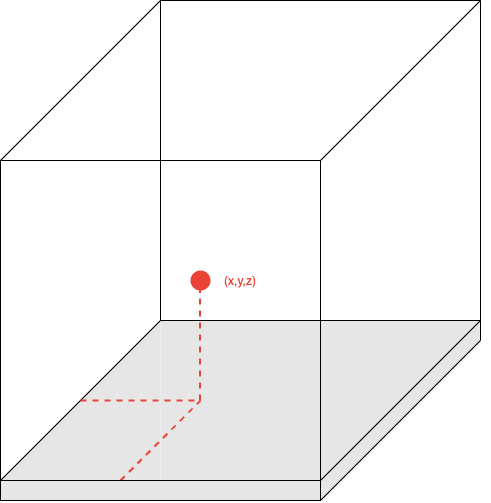
\includegraphics[width=\linewidth]{chapters/chapter2/img/motionPlanning/3DPointConfiguration.png}
    \caption{A robot represented by just a point in 3D space, requiring only 3 Cartesian coordinate $(x,y,z)$ points to describe its \gls{configuration}}
    \label{subfig:3DPointConfig}
    \end{center}
    \end{subfigure}
    &
    % 
    % Subfigure B
    \begin{subfigure}{0.4\textwidth}
    \begin{center}
    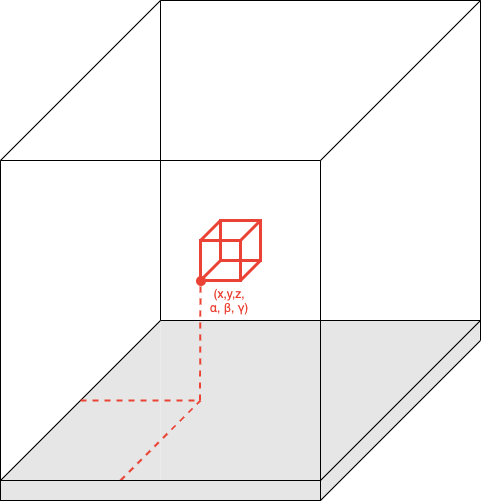
\includegraphics[width=\linewidth]{chapters/chapter2/img/motionPlanning/3DCubeConfiguration.png}
    \caption{A robot represented as a cube in 3D space, now requiring 3 Euler angles $(\alpha, \beta, \gamma)$ along with the original Cartesian coordinates.}
    \label{subfig:3DCubeConfig}
    \end{center}
    \end{subfigure} \\
\end{tabular}
    % Caption and Label
    \caption{Example of 2 Robot Configurations in 3D Space for Motion Planning Purposes}
    \label{fig:configuration}

\end{center}
\end{figure}

